\chapter{Validation}

In the following chapter we'll discuss the results of the formerly
presented implementation, highlighting the benchmarks of the solutions proposed.
In the first part of the chapter we'll investigate the performance of the machine learning
library, in the various situation that may happen. In the following part we will
test the advantages of our microservice oriented architecture with the classical approach
for integration.

\section{Validating Speaker Recognition}

This section is dedicated to the various tests to investigate
the effectiveness in a home security scenario. For our
tests we used two different libraries, comparing their results:
\textit{voiceid} for speaker diarization and identification, \textit{recognito}
for speaker identification only. Furthermore we have used standard configurations
for all the audio files: .wav format, with a frequency 48 kHz and using 16 bit for sampling.

\subsection{Testing the basic model}

Before starting with more complex test it is mandatory to see the effectiveness
of the models in the optimal situation. For the optimal situation we'll take
a unique recording dividing it in the typical machine learning split: 80\% learning
and 20\% for testing the model.\newline
The first test will focus on a batch of voices taken from different sources:

\begin{itemize}
    \item Youtube -  A youtuber using High Quality input camera, using a model with a duration of 50 seconds.
    \item The integrated microphone in my laptop using a model with a duration of 16 seconds.
    \item Voice recordings from Voxforge using a model with a duration 32 seconds.
\end{itemize}
In this scenario the model audio durations will be of different durations and different
quality, we will make more specific tests later in the document.

\subsubsection{Results}

\begin{table}
    \label{tab:basicres}
\centering
\caption{Basic test results}
\begin{tabular}{|c|c|c|c|} \hline
& \textbf{Score \%} & \textbf{Avg Execution (ms)} & \textbf{Avg Duration (s)}\\ \hline
\textbf{Youtuber} & 92.7 & 3217 & 56 \\ \hline
\textbf{Myself} & 81.75 & 2524 & 9.25  \\ \hline
\textbf{Voxforge} & 100 & 2665 & 5.5  \\ \hline
\end{tabular}
\end{table}

As can be seen in \ref{tab:basicres}, the \textit{recognito} library works as expected with
different sources and different quality, proving its correctness for the basic functionalities.
However, we can see a difference in the score of the results depending from the source of the
audio recording. The less quality input, the microphone, has a lower score percentage which is very likely
due to the input quality. It is indeed interesting to notice the perfect score of the audios
taken from \textit{Voxforge}. Although their quality is lower than the Youtube video, their
precision is remarkably high. It is also important to notice the discrepancy between the model
audio durations, which doesn't seem to be affect the score too much. We'll try
to see which is the best duration for a model in the next subsection.

\subsubsection{Finding the optimal length for a Model}

The audio recordings used as model in the former chapter are all of different durations.
However, in order to have a more refined comparison we need to know the best duration of a model
for the best match.\newline
The test will be executed trimming the audio model file in different slots of time, relatively:
1 second, 3 seconds, 5 seconds, 10 seconds and 15 seconds. The models are the same ones
from the previous test.
\pgfplotsset{width=10cm,compat=1.9}

\begin{center}


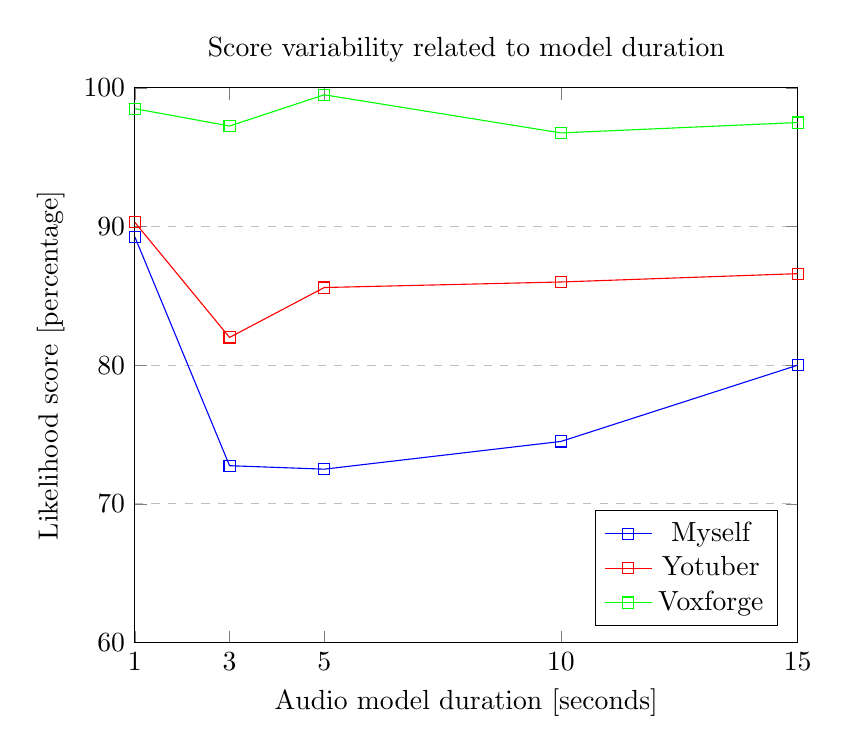
\begin{tikzpicture}

\begin{axis}[
    title={Score variability related to model duration},
    xlabel={Audio model duration [seconds]},
    ylabel={Likelihood score [percentage]},
    xmin=1, xmax=15,
    ymin=60, ymax=100,
    xtick={1,3,5,10,15},
    ytick={60,70,80,90,100},
    legend pos=south east,
    ymajorgrids=true,
    grid style=dashed,
]

\addplot[
    color=blue,
    mark=square,
    ]
    coordinates {
    (1,89.25)(3,72.75)(5,72.5)(10,74.5)(15,80)
    };
\addplot[
    color=red,
    mark=square,
    ]
    coordinates {
    (1,90.3)(3,82)(5,85.6)(10,86)(15,86.6)
    };
\addplot[
    color=green,
    mark=square,
    ]
    coordinates {
    (1,98.5)(3,97.25)(5,99.5)(10,96.75)(15,97.5)
    };
    \legend{Myself,Yotuber,Voxforge}

\end{axis}
\end{tikzpicture}
\end{center}

Surprisingly, as can be seen in the chart above, we had the best results with the
1 second audio model duration. However it is not a good choice to consider this length,
which in some test recordings led to a mismatch in the speaker match. This was more clear
when considering different people from a low quality input (the laptop's microphone),
matching 2 times the wrong person. The mismatch didn't occur with the longer audio models.
It is also interesting to note the fall of the likelihood score for all the models when considering
a slightly longer duration for the audio. This is can be attributed to the noise introduced into the learning process
by some silence in the recording, altering the identification process. The matching
rate starts increasing and slowly normalizing to the optimal matching value approximately
between 10 and 15 seconds.\newline
Despite the fact that this time we used same duration audio models, the test audio segments
were each one of a different duration. In the next section we'll test which is the best duration
for a segment to perform a good match, using the 15 seconds model as the best for our situation.

\subsubsection{Finding the optimal length for an Audio Segment}

As introduced in the previous sections in our scenario we decided to split a single
long audio recording in smaller segments. The question is now to find the optimal duration
for a segment. We will use as model each relative optimal from the previous test, and apply to them
various test model of the following duration length: 1 second, 3 seconds, 5 seconds, 7 seconds,
11 seconds and 13 seconds.

\begin{center}


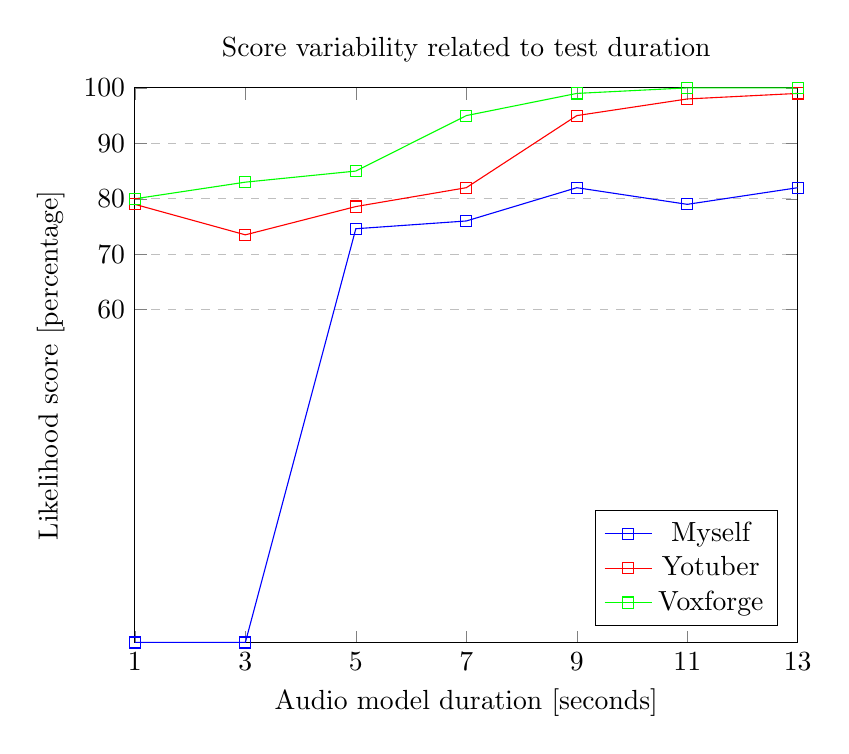
\begin{tikzpicture}

\begin{axis}[
    title={Score variability related to test duration},
    xlabel={Audio model duration [seconds]},
    ylabel={Likelihood score [percentage]},
    xmin=1, xmax=13,
    ymin=0, ymax=100,
    xtick={1,3,5,7,9,11,13},
    ytick={60,70,80,90,100},
    legend pos=south east,
    ymajorgrids=true,
    grid style=dashed,
]

\addplot[
    color=blue,
    mark=square,
    ]
    coordinates {
    (1,0)(3,0)(5,74.6)(7,76)(9,82)(11,79)(13,82)
    };
\addplot[
    color=red,
    mark=square,
    ]
    coordinates {
    (1,79)(3,73.5)(5,78.6)(7,82)(9,95)(11,98)(13,99)
    };
\addplot[
    color=green,
    mark=square,
    ]
    coordinates {
    (1,80)(3,83)(5,85)(7,95)(9,99)(11,100)(13,100)
    };
    \legend{Myself,Yotuber,Voxforge}

\end{axis}
\end{tikzpicture}
\end{center}

As can be seen from the chart, the matching increases linearly with the test duration
length, approaching the best value at 13 seconds.\newline
For short test models the system is unpredictable, though providing generally some
good matches we have noticed some mismatches (marked as 0) for low level inputs. Moreover
these short tests (1 or 3 seconds) seems to be heavily influenced by external noise.\newline
It is also interesting to notice that the running time for the identification process is very slightly
influenced by the length of the duration. This led us to the conclusion that the \textit{13 seconds}
audio duration is the optimal one for our scenario.\newline
Up to now we have used models with different speakers but also from different types of sources. In the
next section we will investigate how the system works when using models applied to the same
speaker but from a different audio source.

\subsection{Testing different inputs with the same speaker}

\subsection{Testing same speaker talking different languages}

\subsection{Animal Identification}
\subsection{Mimic a person}

\subsection{Step Recognition}
